\chapter{Implementation}\label{chap:Algorithms}
\section{Baseline Team Implemenation} 
In this section, I will describe the addtional features described in the Techinical Specification draft and the implementation we made in the OpenUH compiler. 
Previously, we implemented support for Fortran coarrays in OpenUH in accordance with the Fortran 2008
specification~\cite{EachempatiCoarray2013}~\cite{EachempatiCAF2010}.  The OpenUH Coarray Fortran implementation is depicted in Figure~\ref{fig:teams-openuh}.  

\begin{figure}[!h]
\centering
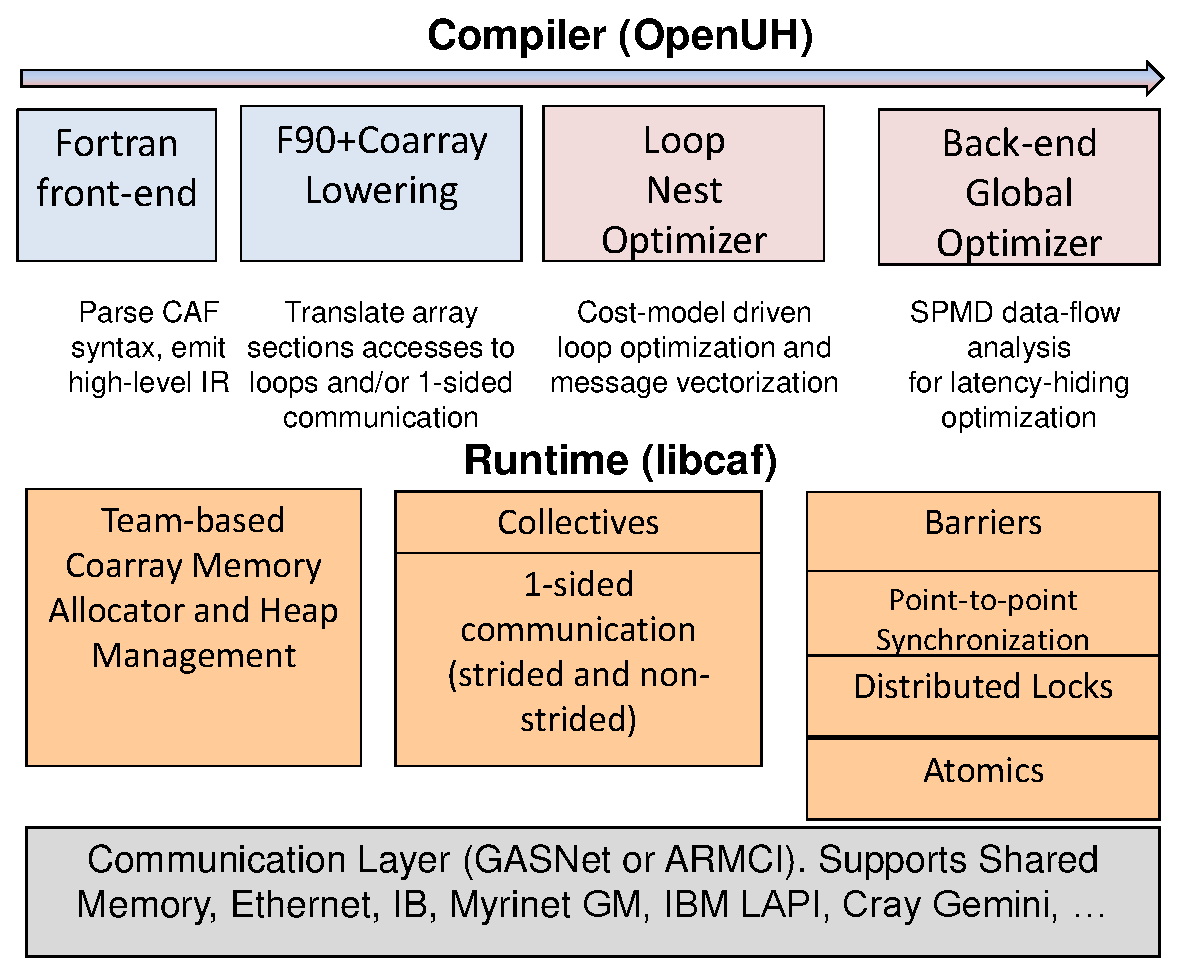
\includegraphics[width=5in, height=4in]{figures/uh-coarrays-implementation-stack.eps}
% where an .eps filename suffix will be assumed under latex, 
% and a .pdf suffix will be assumed for pdflatex; or what has been declared
% via \DeclareGraphicsExtensions.
\caption{OpenUH Coarray Fortran team implementation}
\label{fig:teams-openuh}
\end{figure}

%\subsection{Runtime Design and Implementation for Teams} 

We added support into the Fortran front-end of OpenUH for parsing the
\texttt{form team},  \texttt{change team}, \texttt{end team} and \texttt{sync
team} constructs. We added the new type \texttt{team\_type} to the type system
of OpenUH and support for \texttt{get\_team} and \texttt{team\_number} intrinsics.
We also extended  the CAF intrinsics \texttt{this\_image},
\texttt{num\_images}, and \texttt{image\_index} for teams.
During the back-end compilation process in OpenUH, team-related constructs are
lowered to subroutine calls which constitute the \textit{libcaf} runtime
library interface. In the runtime, we added a \texttt{team\_type} data structure
for storing image-specific identification information, such as the mapping
from a new index to the process identifier in the lower communication layer.
The runtime also provides support for the team-related intrinsics
\texttt{get\_team} and \texttt{team\_number}.


Before team support was added into our implementation, coarray allocation was
globally symmetric across all images, with each coarray allocated at the same
offset within a managed symmetric heap.

With teams, however, this global symmetry is no longer necessary. According to the
draft of the technical specification, symmetric data objects have the
following features, which simplify the memory management for teams. First,
whenever two images are in the same team, they have the same memory
layout. Second, an image can only change to the initial team or teams formed
within  the current team. Third, when exiting a given team, all coarrays
allocated within this team should be deallocated automatically. And fourth, if
an image needs to refer to a coarray of another image located in a sibling
team, the coarray should be allocated in their common ancestor team.

Team variables are opaque, first-class objects which may be used to query
information for a specified team or change to a specified team. In our
implementation, a team variable refers to an associated team data structure,
depicted in Table~\ref{team-ds}. During the formation of a team, the values
for the fields of this data structure are computed and populated, including
(1) the list of images that are on the same node, (2) the number of images
within the same node, and (3) fields used to facilitate execution of
collective operations.  This information is used many times in the runtime by
different parallel algorithms (for example, collectives and barriers as
described in Section~\ref{sec:collectives}).
\begin{table}[!h]
%\begin{minipage}{1\columnwidth}%{\columnwidth}
%\centering

\caption{Team data structure}
\label{team-ds}
%\centering
%\hspace*{0.5in}

\begin{tabular}{|c|L{4.2in}|}
\hline
\textbf{Field} & \textbf{Description}  \\ 
\hline

 team\_num          & a team number or id, assigned during \texttt{form team} statement\\ \hline
 this\_image        & image index for current image in team \\ \hline
 num\_images        & number of images in team \\ \hline
intranode\_set      & ordered list of image indices in same compute node\\\hline
leader\_set         & ordered list of image indices of node leaders in team\\\hline
 leaders\_count     & number of node leaders in team\\\hline
 image\_index\_map  & maps image index to image index in inital team\\ \hline 
 sibling\_maps      & image index mapping for each sibling team created by same \texttt{form team} statement \\\hline
 bar\_parity                  & parity variable for dissemination barrier\\\hline 
bar\_sense                   & sense variable for dissemination barrier\\\hline
intranode\_bar\_flags        & direct shared pointers to intra-node barrier partners' flags\\\hline
bar\_rounds\_info            & partner information for inter-node in dissemination barrier rounds \\\hline
coll\_sync\_flags            & bcast, reduce, and allreduce sync flag\\     \hline
allreduce\_bufid             & selects between two allreduce buffers\\\hline
 reduce\_bufid                & selects between two reduce buffers\\\hline
 bcast\_bufid                 & selects between two bcast buffers \\\hline
 allocations     & a list of symmetric memory slots allocated for this team\\\hline 
 parent  		 & pointer to parent team structure\\\hline
\end{tabular}


\end{table}

\subsection{Memory Management}\label{sec:mm}

\begin{figure}[!h]
\centering
\begin{subfigure}{\textwidth}
	\centering
	\includegraphics[width=.55\linewidth]{figures/memory_step1_nt}
	\caption{Step 1: Allocate Coarray in initial team}
	\label{fig:mm_step1}
\end{subfigure}
\begin{subfigure}{\textwidth}
	\centering
	\includegraphics[width=.55\linewidth]{figures/memory_step2_nt}
	\caption{Step 2: Form new team A and allocate Coarray on image 1, 2}
	\label{fig:mm_step2}
\end{subfigure}
\begin{subfigure}{\textwidth}
	\centering
	\includegraphics[width=.55\linewidth]{figures/memory_step3_nt}
	\caption{Step 3: Form new team B and allocate Coarray on image 1}
	\label{fig:mm_step3}
\end{subfigure}
\begin{subfigure}{\textwidth}
	\centering
	\includegraphics[width=.55\linewidth]{figures/memory_step4_nt}
	\caption{Step 4: End team, exitting from team B}
	\label{fig:mm_step4}
\end{subfigure}
\caption{Evolving state of managed heap during team-relative
symmetric allocations}
\label{fig:memory-steps}
\end{figure}


%the asymmetric memory allocation ...
%the memory allocator logic using teams ...
%Edited by Gracia

Before incorporating support for teams, we implemented the managed heap as
follows. At the beginning of the program, the images collectively allocate a
pinned and registered memory segment which may be used for remote memory
accesses.  Static data which is allocated for the entire lifetime of the
program is placed in a reserved space at the top of this segment. The rest of
the segment is treated as a managed heap. Allocatable coarrays are
symmetrically and synchronously allocated on all images from the top of this
heap. We also allow non-symmetric allocations from the bottom of the heap.
This serves a few different purposes. We can allocate temporary communication
buffers from the bottom and avoid the cost of pinning and registering it.
Additionally, even though Fortran 2008 requires all coarrays to be symmetric
across all images, the coarrays may indirectly point to non-symmetric data.  This is
achieved by declaring the coarray to be of a derived data type with a pointer
or allocatable component, for which the target data may be allocated
independently of other images. This allocated data may then be remotely
referenced using the coarray.

In order to support coarray allocation with respect to teams, we considered a
few different approaches. The first approach was to reserve a
fixed-size memory container for each team, within which any coarray
allocations may be made. This could be achieved, for instance, through the use
of \textit{mspaces} in dlmalloc~\cite{dlmalloc}. However, such an approach
would require foreknowledge of how much space is required for each team, and in
general we expected a considerable waste of allocated space using this
approach.
The second approach which we settled on is to instead reserve a fixed size
heap for all teams except the initial team, which we call the \textit{teams
heap}. This turns out to be sufficient, since a coarray may only be allocated
for a non-initial team when that team is active and none of its descendant
teams have currently allocated coarrays. The initial team is an exception,
since at any time an image may execute a \texttt{change team} statement to
change back to the initial team, and hence a separate heap for the initial team is
still maintained.

\begin{figure}[H]
    \begin{minipage}{0.4\columnwidth}
     \lstset{language=Fortran,basicstyle=\tt\small,
     morekeywords={team, change}
     }
    \begin{lstlisting}
type(TEAM_TYPE) :: I,A,B
integer :: id
integer,allocatable :: d1(:)[:], &
                       d2(:)[:], &
                       d3(:)[:]

I = get_team()
allocate(d1(10)[*])
id = (this_image()-1)/2+1
form team(id, A)
change team(A)
  allocate(d2(10)[*])
  if(team_number() .eq. 1) then
    form team(this_image(), B)
    change team(B)
      allocate(d3(10)[*])
    end team !exit team B
 end if
end team

\end{lstlisting}
\end{minipage}
\caption{Code depicting allocation of coarrays inside teams}
\label{fig:demo-code}
\end{figure}




Figure~\ref{fig:memory-steps} illustrates how our managed heap
evolves over the course of the example program shown in Figure~\ref{fig:demo-code}.
When a coarray is allocated while executing a \texttt{change~team} block, corresponding
allocations should occur on all other images in the \textit{current} team,
rather than for all images.  Upon exiting the \texttt{change~team} block, any
allocations that had occurred within it are implicitly freed if they were not
already freed by a \texttt{deallocate} statement. An image may only
\textit{change} to a team with the \texttt{change team} construct if it was
formed by its current team with a \texttt{form team} statement or if it is the
initial team. The latter scenario requires that the state of symmetric
allocations belonging to the initial team should not be affected by
allocations (not yet freed) belonging to a non-initial team. To support this,
we reserve a fixed section of memory from the top of our managed heap for
symmetric allocations by a non-initial team. 
We divide the list structure for memory allocations into two lists: one is
for symmetric allocations by any non-initial team, and the other is for
symmetric allocations by the initial team and all non-symmetric allocations.
When changing to a new team, the \textit{allocations} field in the team
structure will be set to the current position in the non-initial team
allocations list.

\subsection{Forming and Changing Teams}

%We implement \texttt{form team}, \texttt{change team} and \texftt{end team} in runtime. 

The \texttt{form team} statement forms multiple teams by subdividing the set
of images that are members of the current team. Each image in the current
team must call the statement, specifying the number of the new team it will
join and a team variable which it may use to refer to the newly formed team. A
third optional argument may be specified to request a particular image index
within the new team. It is otherwise implementation-defined how these image
indices are assigned to team members; in our implementation, image indices are
assigned to each image in the order of their indices in the current team.

Forming a new team entails a coordinated exchange of information from every
image in the current team. Our implementation is currently as follows. All the
images collectively perform an \textit{allgather} operation to exchange the
specified team numbers and (if given) image indices. Once this step completes,
each image can determine the members (and their respective image indices) for
each team formed. Based on this, each image can fill in the relevant
information in the team data structure which it associates with the newly
formed team. If a requested image index was specified with the \texttt{form
team} statement, this can be directly assigned to the \textit{this\_image}
field. Otherwise, the new image index is determined by sorting the set of
image indices which specified the same team number. The
\textit{image\_index\_mapping} field is a pointer to an array which maps an
image's image index in the new team to its image index in the initial team.
The leader set contains the image indices for images in the team serving as designated leaders
for their respective compute nodes. The intra-node set contains the
image indices for all images in the team that share the same compute node.
The leader set and intra-node set may be computed based on the runtime's
determination of the process-to-node layout for the job. The \textit{siblings}
field, shown in Table~\ref{team-ds}, is a pointer to an array of image maps
for every other new team formed. This is useful because an image may also
access a coarray belonging to a different team, using an extension to the
normal image selector syntax (e.g., $a[i, team\_number=2]$).  

During the team formation step, we also allocate various synchronization flags
to be used for team-based barriers and collective operations. For barriers, we
distinguish flags to be used for synchronization within a node via shared
memory (available through \textit{intranode\_bar\_flags}),
versus flags used to synchronize between images on separate nodes (available
through \textit{bar\_rounds\_info}). These flags are also stored in the team
data structure associated with each team, shown in Table~\ref{team-ds}.
Pointers for accessing a partner image's
synchronization flag at each round of the barrier are also precomputed and
stored at this stage.
%Another important aspect of the team data structure is to assess which
%information it should maintain that is associatd only to this team. For
%instance, the barrier is associated with specific team, so team need to keep
%track of barrier's status. In form team, it need initialize barrier\_field,
%showed in table~\ref{team-ds}. 
Synchronization flags are also allocated and reserved for supported collective
operations (specifically, \textit{allreduce}, \textit{reduce}, and
\textit{broadcast}) that may be executed by the new team. This is necessary since we implement
collectives using 1-sided communication which is decoupled from
synchronization. Since these collectives entail different communication
structures, in order to allow for their execution to partially overlap we
allocate a distinct set of synchronization flags for each type during team
formation. %More details on our support for team-based collectives and barriers
%are given in Section~\ref{sec:collectives}.

%In previous work, we have developed the memory heirarchy-awared method to
%boost the performance of communication\cite{cafteams-cluster}. The
%\texttt{team} data structure keeps track of the underlying memory structure to
%perform the 2 level algorithms.

%As we described in Section~\ref{sec:mm}, the \texttt{team} is associated with
%a portion of symmetric memory. It can not be determined when \texttt{form
%team} is called since \texttt{form team} and \texttt{change team} can be
%called in different phrase in program. The Coarray allocation between them is
%still associated with the origin team.
%
%To exit from certain team, \texttt{end team} is called. It resets the global
%environment variable to its parent team and marks this team as inactive. Team
%data structure will be freed after its parent has been disabled.

The \texttt{change team} statement is used to change the \textit{current team}
in which the encountering image is executing to a team referenced by a team
variable argument. When an image executes this statement in our
implementation, it will simply change an internal \textit{current\_team}
pointer to the address of the team structure referenced by the team variable.
Next, all images changing to the same team will synchronize via an implicit
team barrier (note that the program should generally ensure that
all or none of the images in a team reach the statement, though its possible
for an image to check for stopped or failed images during its execution). When
\texttt{end team} is encountered, the runtime will set the internal
\textit{current\_team} to point to the parent of the current team. If leaving
a team which has itself created child teams, then the team structures
allocated for each of those child teams may be freed, and the corresponding
team variable will be set to a \texttt{NIL} value to indicate that it is no
longer associated with a team. If the team had allocated coarrays out of the
symmetric heap, the associated slots describing these allocations (in the
\textit{allocations} field) are freed.  Finally, all images in the team it
returns to must synchronize via an implicit team barrier. Note that whenever
an image switches to a different team, through the \texttt{change team} or
\texttt{end team} statements, it will always synchronize will all images which
are members of that team. This ensures that an image will never be executing
in a team while other members are executing in a different team. We make use
of this fact in the synchronization-avoidance optimizations we implemented for
collectives.

\section{Runtime Data Locality Optimization}
In order to make applications more scalable when running on nodes with many cores, the runtime should have some knowledge about the mapping of images on nodes and/or  cores.  If teams create subsets of images, there is no simple relationship between the image structure and the actual  underlying physical structure of the parallel system. Therefore, as a research methodology towards an efficient implementation of  teams, we propose to introduce a memory hierarchy-aware runtime for PGAS, in order to optimize communications within teams via the distinction between local and remote memory accesses.

\section{Optimizing Team Structure}

\subsection{Distributed member mapping list}

%\section{Extensions}
%[in progress]
%\subsection{Non-blocking Team Construct}
%\subsection{Node Team}
%Node team is a kind of teams runtime constructs for users. A node team represent a collect of processes that share the same `Node', usually means they shared the same memory. This can be useful for users to implement better program with considering the data locality. 
